\chapter{Spécification des composants}

\minitoc

\section{Introduction}

	\subsection{Objectif}
Notre architecture étant conséquente, nous devons déterminer les différents composants du système et leur assemblage, afin d'en avoir une meilleur perception.
Notre point de vue se situe à un haut niveau, afin de décrire les exigences de chaque composant.
Il ne s'agit pas pour l'instant de savoir comment sera constitué chacun des composants.

	\subsection{Organisation du chapitre}
%Cette section décrit le contenu du reste du chapitre  et explique comment le document est organisé.
Dans un premier temps, nous essaierons de présenter chacun des composants principaux du système.
Nous aborderons ensuite les différentes interactions entre les composants par le biais de cas d'utilisation.
Nous devrons enfin spécifier les interfaces des différents composants, et spécifier les types d'objets qu'il nous sera nécessaire de créer.

\section{Description des composants}

%Établir les frontières du système.
Une des partie les plus délicates est de définir les frontières entre les différents concepts.

Nous avons choisi de définir un composant ControleCentral qui régit l'ensemble du programme.
Ce composant sera chargé d'utiliser les services fournis par d'autres composants internes.
Nous appellerons ces différents composants: Authentification, Gestionnaire de persistance et MethodeGTD.
Ces trois composants forment une base de l'application, qui devra néanmoins être étoffée pour obtenir un système complètement fonctionnel.
Un composant doit nous permettre la communication avec le serveur. Nous le nommerons donc CommunicationServeur.
Nous aurons également besoin d'un autre composant qui sera chargé du cryptage des données et du hachage du mot de passe, que ce soit en local sur la machine, ou pour la communication avec le serveur distant\footnote{si le serveur nous permet d'utiliser ce genre de fonctionnalités}.

Voyons maintenant cela plus en détail.

%Division du système en composants.

L'agencement des différents composants est décrit dans le schéma ci-dessous : 

\begin{figure}[htbp]
	\centering
		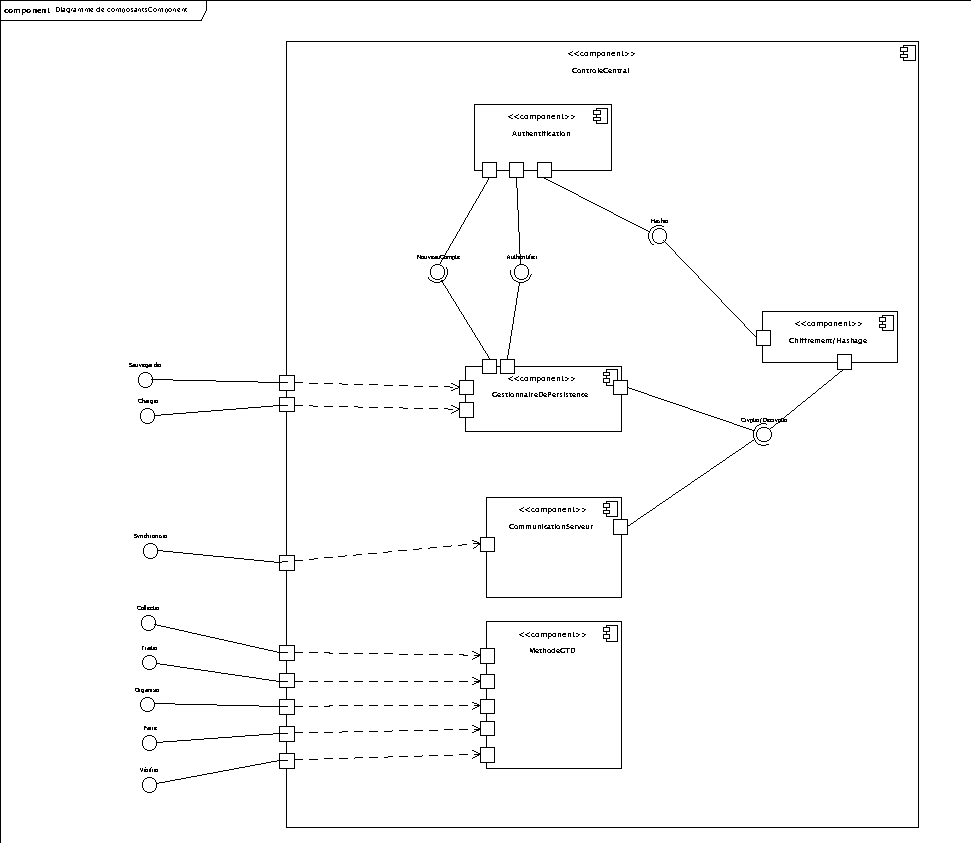
\includegraphics[width=15cm]{images/L3/composants.png}
	\caption{Le composant ControleCentral et ses interfaces}
	\label{fig:ControleCentral}
\end{figure}

%Décrire le comportement souhaité des composants.

\subsection{Le composant ControleCentral}

Voici le composant ControleCentral et les interfaces des services qu'il fourni.
C'est par lui que devront transiter toutes les méthodes.
Cela permettra de garder une gestion cohérente du système. %, en évitant à un futur développeur de créer un controleur .
Nous avons choisi de représenter ce composant global car il nous paraissait évident de le faire figurer, mais nous ne pouvions pas en faire un composant extérieur aux autres car il ne fourni aucune interface, il se contente d'organiser ses composants interne.
Il s'agit donc plus d'une configuration qu'un composant, car il contient tous les autres composants du système.

\subsection{Le composant MethodeGTD}

C'est le composant principal du système.
Il permet d'effectuer les différentes opérations de la méthode GTD sur la structure de donnée.

\subsection{Le composant Chiffrement/Hachage}

Ce composant aura deux tâches bien distinctes : 

\begin{enumerate}
\item il permettra le chiffrement des données pour la sauvegarde des fichiers en local, ainsi que pour la communication avec le serveur.
\item il permettra également le hachage des mots de passe, afin que ceux-ci ne puissent être dévoilés.
\end{enumerate}


\subsection{Le composant Authentification}

%Comme son nom l'indique, ce composant permettra l'authentification des différents utilisateurs du système.
Cet outil devant pouvoir être utilisé potentiellement par plusieurs utilisateurs, le système aura besoin d'un composant capable de gérer les authentifications de chacun d'eux.
Il doit donc permettre d'indiquer si un mot de passe donné est bien celui correspondant au login de l'utilisateur.

\subsection{Le composant GestionnaireDePersistence}

Le système devant pouvoir être utilisé uniquement de manière locale, nous devons pouvoir gérer la persistance des données, de manière à ce que l'utilisateur puisse éteindre son ordinateur par exemple.
Nous devrons alors enregistrer notre structure de donnée sous forme de fichier.
Ce composant aura aussi la responsabilité de charger les données d'un utilisateur contenues dans la base, après avoir vérifié son login et mot de passe.

\subsection{Le composant CommunicationServeur}

Ce composant a été défini afin de pouvoir communiquer avec le serveur.
Il devra permettre la synchronisation des données entre le client local et le serveur distant, par le biais d'une communication cryptée.
La représentation des données n'étant pas forcément identique entre le client et le serveur, le composant devra donc effectuer un travail de conversion des données.




\section{Interactions}

Dans ce qui suit, nous allons décrire les interactions principales entre les principaux acteurs de notre système.
On se focalisera en particulier sur les cas d'utilisation qui seront le plus souvent rencontrés.

%Décrire, à haut-niveau, la collaboration entre les composants majeurs, en faisant référence aux besoins.
Voici, à haut niveau, la manière dont les différents composants collaborent entre eux.
// 
Toutes les actions sont initiées par le composant ControleCentral( avec lequel interagira l'utilisateur). Les opérations complexes sur le compte actif sont effectuées par le composant MethodeGTD, mais la persistance des modifications est lancée par ControleCentral, et effectuée par le gestionnaire de persistance.
Le chargement d'un compte utilisateur est effectuée par le gestionnaire de persistance. Celui-ci utilise le composant Authentification, pour savoir quel compte charger, et le composant Chiffrement, pour décrypter les données stockées.//
L'authentification utilise également le composant Chiffrement(ou du moins sa fonction de hachage), afin de comparer le login et le mot de passe entrés avec ceux existants.
Enfin, le composant CommunicationServeur utilise également le Chiffrement pour crypter la communication distante.



%Utiliser des interactions, c'est à dire, des diagrammes de séquence et des diagrammes de communication. Utiliser éventuellement des diagrammes d'activités.

%\emph{Ne vous limitez pas à une seule interaction par cas d'utilisation}

\subsection{Traiter une chose a faire }

\begin{figure}[!htbp]
\centering
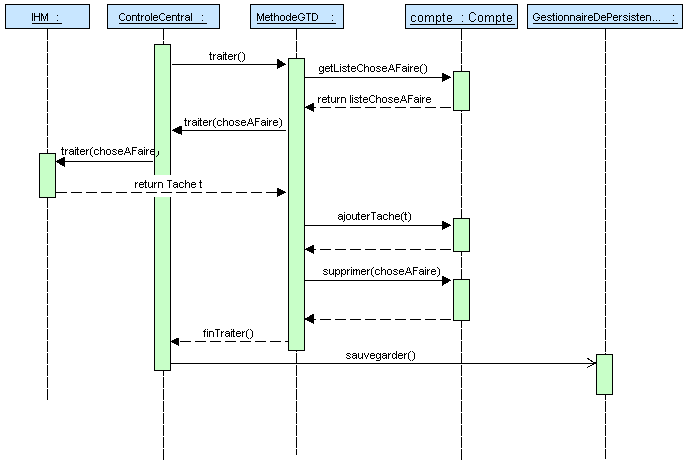
\includegraphics[width=12cm]{images/L3/diagrammeSequence/Traiter.png}
\caption{Interaction \--- Traiter \-- Création d'une tâche}
\label{traiterSequence}
\end{figure}

Dans le premier diagramme \ref{traiterSequence}  , on peut voir la séquence d'appel intervenant lors du traitement d'une Chose A Faire, lorsque celle-ci donne lieu à la création d'une tâche.
\\
Dans le diagramme suivant \ref{traiterActivite}, on peut voir les différents chemins que peut prendre l'algorithme de traitement. On peut y voir les possibilités de création de projet, sous-projet, projet ordonné(dépendance entre les tâches) etc.


\begin{figure}[!htbp]
\centering
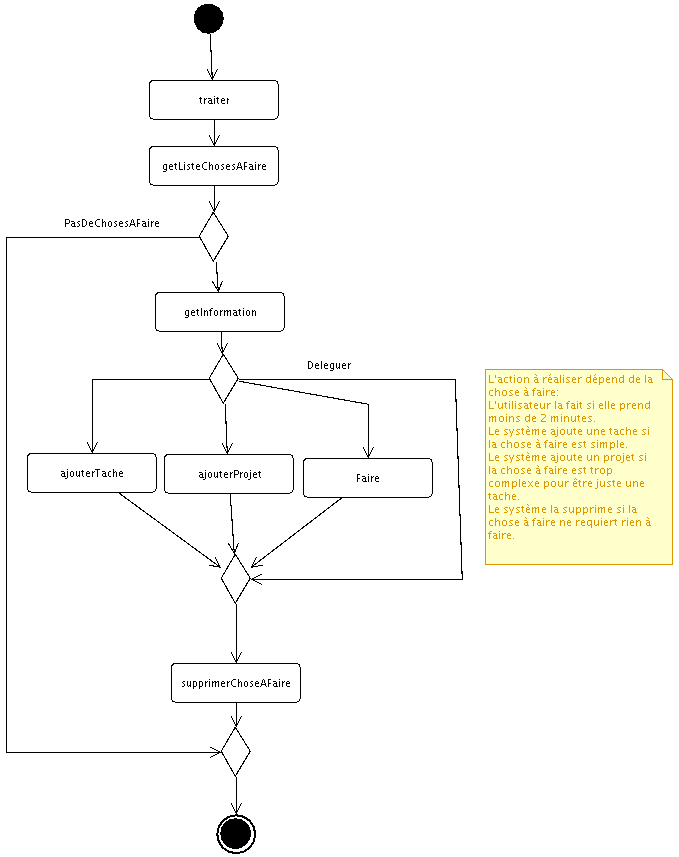
\includegraphics[width=12cm]{images/L3/diagrammeActivite/Traiter.png}
\caption{Interaction \--- Traiter \-- vue générale}
\label{traiterActivite}
\end{figure}

\subsection{Organiser des tâches}

Dans le diagramme \ref{organizeSequence}, on peut observer une séquence du cas Organiser. 

\begin{figure}[!htbp]
\centering
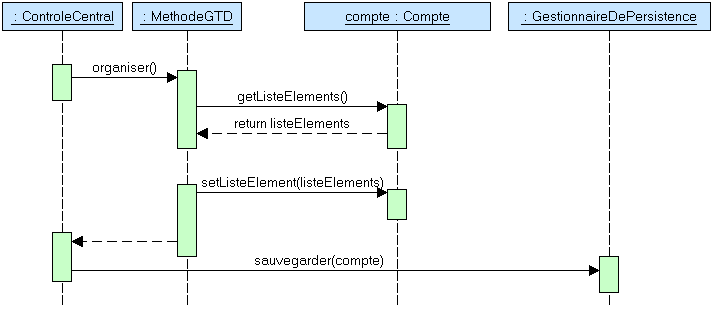
\includegraphics[width=12cm]{images/L3/diagrammeSequence/organiser.png}
\caption{Interaction \--- Organiser}
\label{organizeSequence}
\end{figure}

\subsection{Examen des tâches}

Le diagramme \ref{examinerSequence} représente l'examen des tâches.

\begin{figure}[!htbp]
\centering
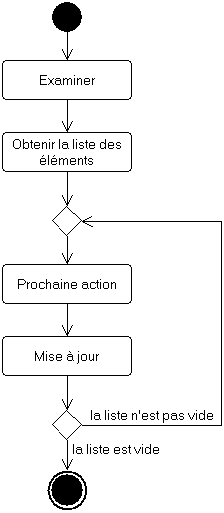
\includegraphics[scale=0.5]{images/L3/diagrammeActivite/examiner.png}
\caption{Interaction \--- Examiner}
\label{examinerSequence}
\end{figure}

\subsection{Faire une tâche}

Le diagramme \ref{doSequence} représente l'action de faire une tâche.

\begin{figure}[!htbp]
\centering
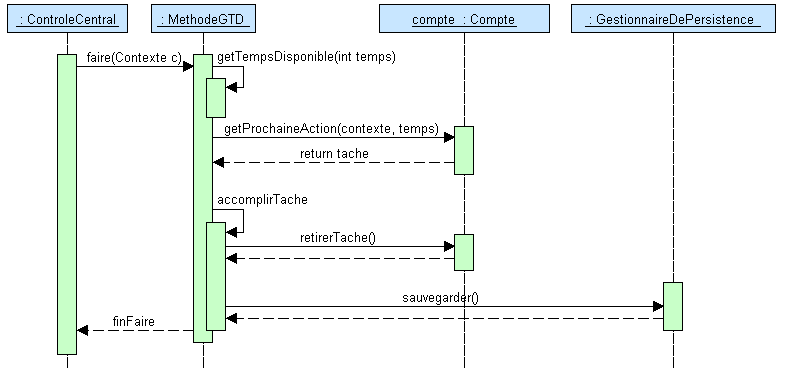
\includegraphics[width=12cm]{images/L3/diagrammeSequence/faire.png}
\caption{Interaction \--- Faire}
\label{doSequence}
\end{figure}

\subsection{Authentification d'un utilisateur}

Le diagramme d'activité \ref{authSequence} représente l'authentification des utilisateurs.

\begin{figure}[!htbp]
\centering
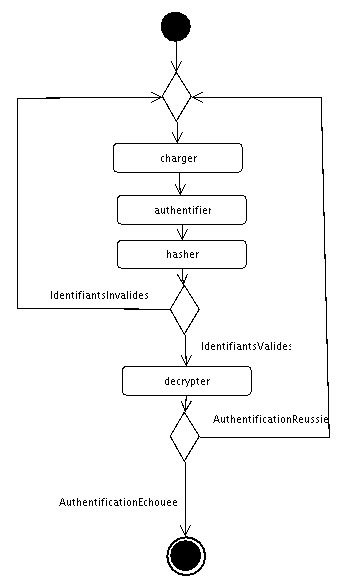
\includegraphics[width=12cm]{images/L3/diagrammeActivite/authentification.png}
%faudrai en faire un...
\caption{Interaction \--- Authentifier}
\label{authSequence}
\end{figure}

\section{Spécification des interfaces}

	\subsection{Interface du composant MethodeGTD}

		\begin{itemize}
			\item \code{collecter(idee : String) : void} \\
			Permet de collecter un nouvelle idée
			\begin{ocl}
-- L'idee doit exister
context collecter(idee : String) : void
pre: idee <> null
	and idee.size()>0
			\end{ocl}

			\item \code{traiter(idee : ChoseAFaire) : Tache} \\
			Renseigne une idée, pour la transformer en tâche.

			\item \code{organiser() : void} \\
			Calcule la priorité dynamique des tâches, et les ordonne selon cette priorité.

			\item \code{verifier(listeTache : Tache[*]) : void} \\
			Passe en revue une liste de tâches, pour mettre à jour la priorité dynamique.

			\item \code{faire(listeTache : Tache[*], contexte : Contexte) : Tache} \\
			Sélectionne la tâche la plus importante à faire selon un contexte donné.
		\end{itemize}

	\subsection{Interface du composant GestionnaireDePersistance}

	L'interface du gestionnaire de persistance autorise le chargement/enregistrement d'un compte à partir/depuis un fichier à l'aide d'un login et d'un mot de passe.

		\begin{itemize}
			\item \code{sauvegarder() : void} \\
			Permet de sauvegarder le compte lié au login de l'utilisateur
			\item \code{charger(login : String, motDePasse : String) : Comptes} \\
			Charge et renvoie le compte lié au login si le mot de passe est correct.
			\item \code{enregistrerIdentifiants(tableCleValeur : Map<String, String>) : void} \\
			Enregistre la table des identifiants et mots de passe cryptés dans un fichier.
			\item \code{chargerIdentifiants() : Map<String, String>} \\
			Charge la table des identifiants et mots de passe cryptés depuis un fichier.
		\end{itemize}

Nous avons définit la fonction sauvegarder comme ceci car le gestionnaire de persistance gardera en mémoire l'identifiant du compte chargé, ou bien pourra le récupérer depuis le contrôle central, qui devra être un singleton.
Nous verrons la meilleure façon de faire lors de l'implémentation.

	\subsection{Interface du composant Chiffrement/Hachage}

	L'interface du ce composant permet le chiffrement et le déchiffrement de fichier ainsi que le hachage (pour des mots de passe typiquement).

		\begin{itemize}
			\item \code{crypter(entree : Fichier) : Fichier} \\
			Crypte un fichier donné dans un autre fichier.
			\item \code{decrypter(entree : Fichier) : Fichier} \\
			Décrypte un fichier donné et restitue un fichier non crypté.
			\item \code{hasher(motDePasse : String) : String} \\
			Crypte le mot de passe de manière unidirectionnel.
		\end{itemize}

Concernant le cryptage/décryptage, nous nous sommes basés sur des fichiers pour l'instant, bien que nous ne sachons pas comment ce système pourra être représenté.
Il pourrait s'agir de transformer un Compte en chaine de caractères cryptée.
Nous verrons cela plus en détail lors de l'implémentation.

	\subsection{Interface du composant Authentification}

	L'interface de ce composant permet l'authentification des utilisateur.

		\begin{itemize}
			\item \code{authentifier(nom : String, motDePasse : String) : boolean} \\
			Authentifie ou non un utilisateur suivant un mot de passe donné.
			\item \code{nouveauCompte(nom : String, motDePasse : String) : void} \\
			Associe un nouvel utilisateur et son mot de passe.
			\begin{ocl}
-- Le nom ne doit pas etre la valeur null.
-- La taille du nom est superieur a 0.
contexte nouveauCompte(nom, motDePasse) : void
pre: nom <> null
	and nom.size > 0
			\end{ocl}
		\end{itemize}


	\subsection{Interface du composant CommunicationServeur}

		\begin{itemize}
			\item \code{synchroniser(compte : Comptes) : void} \\
			Permet de synchroniser l'ensemble des tâches avec le serveur.
		\end{itemize}

\section{Spécification des types utilisés}

Spécifiez ici les types utilisés par les interfaces (seulement ceux qui ne font pas partie des types de base UML).

\subsection{Element, Tache et Projet}

Afin de permettre un traitement identique sur les différentes tâches et projets, nous avons utilisé le patron de conception composite.

\subsubsection{Element}
Nous avons donc défini une classe mère Element, qui contient les attributs et opérations commun aux classes Tache et Projet.

	\begin{description}
		\item[id]: l'identifiant unique de la tâche.
		\item[nom]: le nom de la tâche.
		\item[notes]: la description de la tâche.
		\item[prioriteDynamique]: la priorité calculée par la méthode GTD.
	\end{description}

\begin{figure}[htbp]
	\centering
		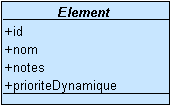
\includegraphics[scale=1]{images/L3/structureDonnee/element.png}
	\caption{La classe Element}
	\label{fig:element}
\end{figure}

\subsubsection{Tache}

	La classe \code{Tache} représente une tâche. Elle possède les attributs suivants:
	\begin{description}
		\item[priorite]: la priorité fixée par l'utilisateur.
		\item[tauxEffort]: le taux d'effort demandé par la tâche.
		\item[liens]: liste des liens internet liés à la tâche.
		\item[tags]: la liste des tags associés à cette tâche.
		\item[isActive]: détermine si la tâche est activée ou non.
	\end{description}

\begin{figure}[htbp]
	\centering
		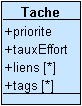
\includegraphics[scale=1]{images/L3/structureDonnee/tache.png}
	\caption{La classe Tache}
	\label{fig:tache}
\end{figure}

\subsubsection{Projet}

Nous avons décidé de spécifier deux types de projets : ordonné ou non.
Un projet ordonné permet de gérer des dépendances entre les tâches qui le composent (par exemple la deuxième tâche dépend de la première d'un même dossier).
Nous avons choisi cette méthode car cela permet d'avoir des dépendances en arborescence, et donc évite les cycles de dépendance qu'il pourrait y avoir si la dépendance n'était qu'un attribut d'une tâche (ou ici d'un élément).
Nous avons donc une classe abstraite Projet, et deux classes concrètes \code{ProjetOrdonne} et \code{ProjetNonOrdonne}.
Chaque classe concrète peut alors choisir la représentation de sa liste interne.

	La classe \code{Projet} représente un ensemble de tâches. Un projet possède les attributs suivants:
	\begin{description}
		\item[listeElement]: les éléments contenus dans  le projet.
	\end{description}

\begin{figure}[htbp]
	\centering
		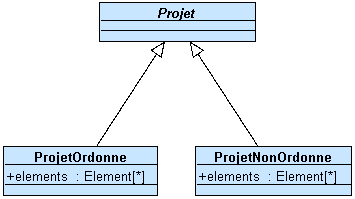
\includegraphics[scale=1]{images/L3/structureDonnee/projets.png}
	\caption{La classe Projet}
	\label{fig:Projet}
\end{figure}

\subsection{Contexte}

	La classe \code{Contexte} représente le contexte associé à une tâche (cf figure \ref{fig:Contexte}). Elle possède les attributs suivants:
	\begin{description}
		\item[nom]: le nom du contexte.
	\end{description}

\begin{figure}[htbp]
	\centering
		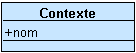
\includegraphics[scale=1]{images/L3/structureDonnee/contexte.png}
	\caption{La classe Contexte}
	\label{fig:Contexte}
\end{figure}

\subsection{Echeancier}

	La classe \code{Echeancier} représente l'échéancier d'une tâche (cf figure \ref{fig:Echeancier}). Elle possède les attributs suivants:
	\begin{description}
		\item[dateDebut]: La date du début de la tâche.
		\item[echeance]: l'écheance de la tâche.
		\item[frequence]: la fréquence de répétition de la tâche.
		\item[dateArret]: la date d'arrêt de la répétition.
	\end{description}

\begin{figure}[htbp]
	\centering
		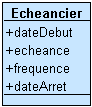
\includegraphics[scale=1]{images/L3/structureDonnee/echeancier.png}
	\caption{La classe Echeancier}
	\label{fig:Echeancier}
\end{figure}

\subsection{Contact}

	La classe \code{Contact} représente les contacts auxquelles les tâches peuvent être associées (cf figure \ref{fig:Contact}). Elle possède les attributs suivants:
	\begin{description}
		\item[nom]: le nom du contact.
		\item[eMail]: son adresse e-mail.
		\item[telephone]: son numéro de téléphone.
		\item[adresse]: son adresse postale.
	\end{description}

\begin{figure}[htbp]
	\centering
		
\includegraphics[scale=1]{images/L3/structureDonnee/contact.png}
	\caption{La classe Contact}
	\label{fig:Contact}
\end{figure}

\subsection{Compte}

La classe \code{Compte} représente le compte auquel est associé un login.
C'est cette classe qui contient l'ensemble des éléments (tâches et projets) d'un utilisateur (cf figure \ref{fig:compte}).
Elle possède les attributs suivants:
	\begin{description}
		\item[nom]: le login du compte.
		\item[mdp]: le mot de passe du compte.
	\end{description}

\begin{figure}[htbp]
	\centering
		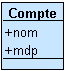
\includegraphics[scale=1]{images/L3/structureDonnee/compte.png}
	\caption{La classe Compte}
	\label{fig:compte}
\end{figure}

\subsection{Ensemble de la structure de donnée}

Voici donc la corrélation des divers éléments de notre structure de donnée (cf figure \ref{fig:structure}).

\begin{figure}[htbp]
	\centering
		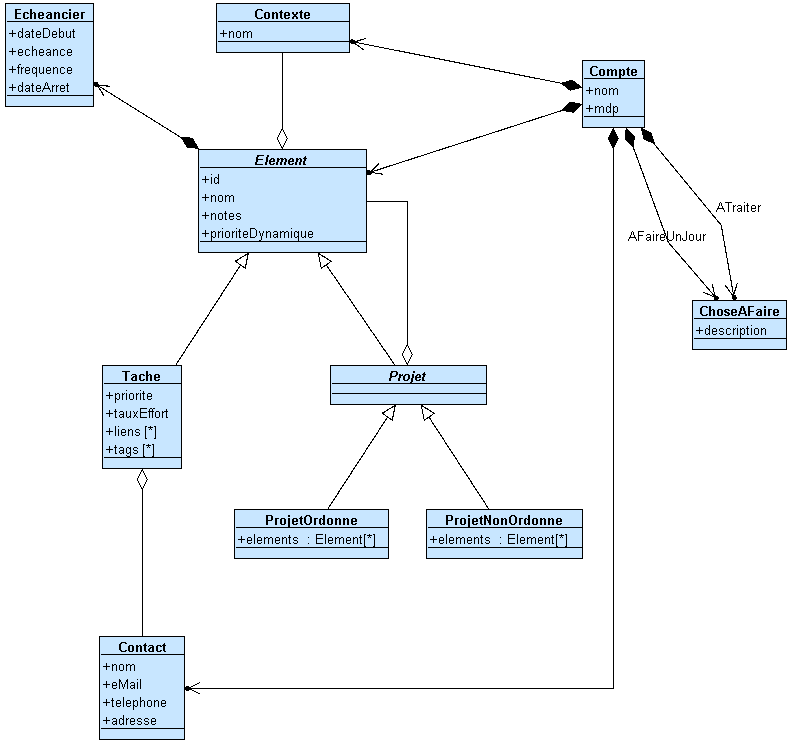
\includegraphics[width=15cm]{images/L3/structureDonnee/comptes.png}
	\caption{La structure de donnée}
	\label{fig:structure}
\end{figure}

\section{Conclusion}

Maintenant que les frontières du système sont établies, nous allons pouvoir détailler chaque composant défini précédemment.
